\section{Modellizzazione}
\subsection{Modelli di flusso continuo - modelli di trasferimento di risorse a tempo continuo}
\subsubsection*{Introduzione}
I modelli a flusso continuo, o modelli di trasferimento di risorse a tempo continuo, sono modelli costituiti da più compartimenti,
in cui si analizzano gli spostamenti delle risorse tra i diversi compartimenti.

\subsubsection*{Rappresentazione grafica}
\begin{center}
	\begin{minipage}{0.4\textwidth}
		\centering
		\includegraphics[width=0.8\textwidth]{modelli/modello flusso continuo.png}
	\end{minipage}
	\begin{minipage}{0.5\textwidth}
		\begin{align*}
			l \;\; &\rightarrow \;\; \text{ingresso } u_l(t) \\
			h \;\; &\rightarrow \;\; \text{uscita } u_h(t) \\
			i \;\; &\rightarrow \;\; \text{compartimento o contenitore di risorse} \\
			j \;\; &\rightarrow \;\; \text{compartimento o contenitore di risorse} \\
			\alpha, \beta, \gamma \;\; &\rightarrow \;\; \text{parametri di flusso } \in \mathbb{R} 
		\end{align*}
	\end{minipage}
	\begin{align*}
		x_i(t) &\rightarrow \;\; \text{risorse nel compartimento } i \text{ all'istante } t, \text{ variabile di stato} \\
		x_j(t) &\rightarrow \;\; \text{risorse nel compartimento } j \text{ all'istante } t, \text{ variabile di stato} \\
		\alpha_{ij} x_i(t) &\rightarrow \;\; \text{trasferimento di risorse dal compartimento } i \text{ al compartimento } j \\
		\alpha_{ji} x_j(t) &\rightarrow \;\; \text{trasferimento di risorse dal compartimento } j \text{ al compartimento } i \\
		\alpha_{i0} x_i(t) &\rightarrow \;\; \text{trasferimento di risorse dal compartimento } i \text{all'ambiente, perdite} \\
		\beta_{li} u_l(t) &\rightarrow \;\; \text{trasferimento di risorse dall'ingresso al compartimento } i \\
		\beta_{ih} u_h(t) &\rightarrow \;\; \text{trasferimento di risorse dal compartimento } i \text{all'uscita} \\
		\gamma_{ii} x_i(t) &\rightarrow \;\; \text{accumulo della risorsa generata nel compartimento } i  \\
		\gamma_{ji} x_j(t) &\rightarrow \;\; \text{trasferimento della risorsa generata in } j \text{ da } j \text{ a } i
	\end{align*}
\end{center}

\subsubsection*{Rappresentazione in funzioni matematiche}
Per ogni compartimento si scrive l'equazione del bilancio del flusso:
\[\text{velocità di variazione delle risorse in } i \;\; = \;\; \text{flusso entrante in } i \;\; - \;\; \text{flusso uscente da } i\]
Si ottengono \(n\) equazioni differenziali, una per ogni \(i\) compartimento (con \(n\) compartimenti):
\[\dot{x}_i(t) \;\; = \;\; \left(\sum_{l=1}^{p} \beta_{li} u_l(t) + \sum_{j = 1 \;\; j \neq i}^{n} (\alpha_{ji} + \gamma_{ji}) x_j(t) + \gamma_{ii} x_i(t)\right) \;\; - \;\; \left(\sum_{h=1}^{p} \beta_{ih} u_h(t) + \sum_{j=0}^{n} \alpha_{ij} x_i(t)\right)\]
È possibile scrivere tutto ciò in forma matriciale: \(\quad \dot{x}(t) = Ax(t) + Bu(t)\)
\[x(t) = \left[\begin{matrix} x_1(t) \\ \vdots \\ x_n(t) \end{matrix}\right]_\text{variabili di stato} \qquad
\dot{x}(t) = \left[\begin{matrix} \dot{x}_1(t) \\ \vdots \\ \dot{x}_n(t) \end{matrix}\right]_\text{variazione var. di stato} \qquad
u(t) = \left[\begin{matrix} u_1(t) \\ \vdots \\ u_p(t) \end{matrix}\right]_\text{entrate/uscite}\]
\[A = \left[\begin{matrix} a_{11} & a_{12} & \dots & a_{1n} \\ a_{21} & a_{22} & \dots & a_{2n} \\ \vdots & \vdots & \ddots & \vdots \\ a_{n1} & a_{n2} & \dots & a_{nn} \end{matrix}\right] \quad
\text{ con } \begin{cases} a_{ij} = \alpha_{ji} + \gamma_{ji} \\[5pt] \displaystyle a_{ii} = \gamma_{ii} - \sum_{j = 0 \;\; j \neq i}^{n} \alpha_{ij} \end{cases} \qquad\qquad\quad
B(t) = \left[\begin{matrix} \beta_{li} \\ \vdots \\ \beta_{ih} \end{matrix}\right] \qquad\qquad\quad\]

\subsubsection*{Punto di equilibrio di un modello a flusso continuo / trasferimento di risorse}
Dato un sistema dinamico nella forma \(\dot{x}(t) = Ax(t) + Bu(t)\), per calcolarne l'equilibrio:
\begin{itemize}
	\item[1.] si fissano gli ingressi e le uscite ad un certo valore \(u(t) = \bar{u}\), altrimenti se gli ingressi continuano
	a variare, non si raggiungerà mai una situazione di equilibrio
	\item[2.] si definisce lo stato di equilibrio \(\bar{x}\) tale per cui \(\bar{x} = x(t)\) per \(t \gg 0\)
	\item[3.] si osserva che all'equilibrio non ci devono essere variazioni delle risorse, ovvero \(\dot{x}(t) = 0\)
	\item[4.] si ottiene un'equazione matriciale \(0 = A \bar{x} + B \bar{u}\) nell'incognita \(\bar{x}\)
	\item[5.] la soluzione dell'equazione corrisponde allo stato di equilibrio e vale: \[\bar{x} = -A^{-1}B \bar{u}\]
\end{itemize}
Si osserva che in un sistema isolato, senza ingressi e uscite, la soluzione dell'equazione \(0 = A \bar{x}\) corrisponde al
nucleo della matrice \(A\): \(\bar{x} = \ker \left\{A\right\}\)


\subsubsection*{Esempi visti a lezione}
\begin{itemize}
	\item serbatoio con ingressi, uscite, serbatoi multipli intermedi e altre variazioni
	\item sistema di raffreddamento della CPU
	\item traffico automobilistico
	\item parco macchine
	\item emigrazione italiana con natalità
\end{itemize}

\newpage

\subsection{Modelli di decisione - modelli di trasferimento di risorse a tempo discreto (istanti privilegiati)}
\subsubsection*{Introduzione}
I modelli di decisione, o modelli di trasferimento di risorse a tempo discreto, sono modelli costituiti da più compartimenti,
in cui si analizzano gli spostamenti delle risorse tra i diversi compartimenti in istanti di tempo privilegiati. Le rappresentazioni
e i procedimenti sono molto simili ai modelli di flusso continuo.

\subsubsection*{Rappresentazione grafica}
\begin{center}
	\begin{minipage}{0.4\textwidth}
		\centering
		\includegraphics[width=0.8\textwidth]{modelli/modello flusso continuo.png}
	\end{minipage}
	\begin{minipage}{0.5\textwidth}
		\begin{align*}
			l \;\; &\rightarrow \;\; \text{ingresso } u_l(k) \\
			h \;\; &\rightarrow \;\; \text{uscita } u_h(k) \\
			i \;\; &\rightarrow \;\; \text{compartimento o contenitore di risorse} \\
			j \;\; &\rightarrow \;\; \text{compartimento o contenitore di risorse} \\
			\alpha, \beta, \gamma \;\; &\rightarrow \;\; \text{parametri di flusso } \in \mathbb{R} 
		\end{align*}
	\end{minipage}
	%\begin{align*}
	%	x_i(k) &\rightarrow \;\; \text{risorse nel compartimento } i \text{ all'istante } k, \text{ variabile di stato} \\
	%	x_j(k) &\rightarrow \;\; \text{risorse nel compartimento } j \text{ all'istante } k, \text{ variabile di stato} \\
	%	\alpha_{ij} x_i(k) &\rightarrow \;\; \text{trasferimento di risorse dal compartimento } i \text{ al compartimento } j \\
	%	\alpha_{ji} x_j(k) &\rightarrow \;\; \text{trasferimento di risorse dal compartimento } j \text{ al compartimento } i \\
	%	\alpha_{i0} x_i(k) &\rightarrow \;\; \text{trasferimento di risorse dal compartimento } i \text{all'ambiente, perdite} \\
	%	\beta_{li} u_l(k) &\rightarrow \;\; \text{trasferimento di risorse dall'ingresso al compartimento } i \\
	%	\beta_{ih} u_h(k) &\rightarrow \;\; \text{trasferimento di risorse dal compartimento } i \text{all'uscita} \\
	%	\gamma_{ii} x_i(k) &\rightarrow \;\; \text{accumulo della risorsa generata nel compartimento } i  \\
	%	\gamma_{ji} x_j(k) &\rightarrow \;\; \text{trasferimento della risorsa generata in } j \text{ da } j \text{ a } i
	%\end{align*}
\end{center}
I parametri \(x_i(k)\), \(x_j(k)\), \(\alpha_{ij} x_i(k)\), \(\alpha_{ji} x_j(k)\), \(\alpha_{i0} x_i(k)\), \(\beta_{li} u_l(k)\), \(\beta_{ih} u_h(k)\),
\(\gamma_{ii} x_i(k)\), \(\gamma_{ji} x_j(k)\) sono analoghi al modello precedente, soltanto che ora, al posto di essere in funzione
del tempo \(t \in \mathbb{R}\), sono in funzione di istanti privilegiati attraverso la variabile \(k \in \mathbb{N}\)

\subsubsection*{Rappresentazione in formule matematiche}
Per ogni compartimento si scrive l'equazione del bilancio del flusso:
\[\text{variazione delle risorse in } i \;\; = \;\; \text{flusso entrante in } i \;\; - \;\; \text{flusso uscente da } i\]
Si ottengono \(n\) equazioni, una per ogni \(i\) compartimento (con \(n\) compartimenti):
\begin{align*}
	&x_i(k\!+\!1) - x_i(k) = \left(\sum_{l=1}^{p} \beta_{li} u_l(k) + \!\!\!\!\sum_{j = 1 \;\; j \neq i}^{n} (\alpha_{ji} + \gamma_{ji}) x_j(k) + \gamma_{ii} x_i(k)\right) - \left(\sum_{h=1}^{p} \beta_{ih} u_h(k) + \sum_{j=0}^{n} \alpha_{ij} x_i(k)\right) \\
	&x_i(k\!+\!1) = \left(\sum_{l=1}^{p} \beta_{li} u_l(k) +  \!\!\!\!\sum_{j = 1 \;\; j \neq i}^{n} (\alpha_{ji} + \gamma_{ji}) x_j(k) + \gamma_{ii} x_i(k)\right) - \left(\sum_{h=1}^{p} \beta_{ih} u_h(k) + \sum_{j=0}^{n} \alpha_{ij} x_i(k)\right) + x_i(k)
\end{align*}
È possibile scrivere tutto ciò in forma matriciale: \(\quad x(k+1) = Ax(k) + Bu(k)\)
\[x(k) = \left[\begin{matrix} x_1(k) \\ \vdots \\ x_n(k) \end{matrix}\right] \qquad
u(k) = \left[\begin{matrix} u_1(k) \\ \vdots \\ u_p(k) \end{matrix}\right] \qquad
B(k) = \left[\begin{matrix} \beta_{li} \\ \vdots \\ \beta_{ih} \end{matrix}\right] \qquad A = \left[\begin{matrix} a_{11} & a_{12} & \dots & a_{1n} \\ a_{21} & a_{22} & \dots & a_{2n} \\ \vdots & \vdots & \ddots & \vdots \\ a_{n1} & a_{n2} & \dots & a_{nn} \end{matrix}\right]\]
\[\text{ con } a_{ij} = \alpha_{ji} + \gamma_{ji} \qquad\qquad a_{ii} = 1 + \gamma_{ii} - \sum_{j = 0 \;\; j \neq i}^{n} \alpha_{ij}\]

\subsubsection*{Esempi visti a lezione}
\begin{itemize}
	\item modello di Leslie a struttura d'età (approfondito successivamente)
	\item fenomeno di emigrazione
	\item sistema di utilizzo della CPU
\end{itemize}

\newpage

\subsection{Modello a struttura d'età - modello di Leslie}
\subsubsection*{Introduzione}
I modelli a struttura d'età o di Leslie sono modelli di trasferimento di risorse a tempo discreto specifici per analizzare l'andamento
di una popolazione, suddividendola in classi d'età. In genere si contano il numero di femmine per classe d'età.

\subsubsection*{Rappresentazione grafica}
\begin{center}
	\includegraphics[width=0.75\textwidth]{modelli/modello leslie.png}
	\begin{align*}
		1,2, \dots n \;\; &\rightarrow \;\; \text{compartimenti / classi di età} \\
		x_1(k) \;\; &\rightarrow \;\; \text{popolazione con età} \in \left[ \; 0, \;T \; \right[ \\
		x_i(k) \;\; &\rightarrow \;\; \text{popolazione con età} \in \left[ \; (i-1)T, \;iT \; \right[ \\
		x_n(k) \;\; &\rightarrow \;\; \text{popolazione con età} \in \left[ \; nT, \; +\infty \; \right[ \\
		s_0 \;\; &\rightarrow \;\; \text{tasso di sopravvivenza alla nascita} \in \mathbb{R} \\
		s_i \;\; &\rightarrow \;\; \text{tasso di sopravvivenza per passaggio alla classe successiva} \in \mathbb{R} \\
		f_i \;\; &\rightarrow \;\; \text{tasso di fertilità} \in \mathbb{R} \\
		1-s_i \;\; &\rightarrow \;\; \text{tasso di mortalità} \in \mathbb{R}
	\end{align*}
\end{center}

\subsubsection*{Rappresentazione in formule matematiche}
Per il primo compartimento si ha:
\[x_1(k+1) - x_1(k) = s_0 \sum_{i=1}^{n} f_i x_i(k) - s_1 x_1(k) - (1-s_1) x_1(k) \qquad \rightarrow \qquad x_1(k+1) = s_0 \sum_{i=1}^{n} f_i x_i(k)\]
Per un generico compartimento \(i\) con \(1 < i < n\) si ha:
\[x_i(k+1) - x_i(k) = s_{i-1} x_{i-1}(k) - s_i x_i(k) - (1-s_i)x_i(k) \qquad \rightarrow \qquad x_i(k+1) = s_{i-1} x_{i-1}(k)\]
Per l'ultimo compartimento si ha:
\[x_n(k+1) - x_n(k) = s_{n-1} x_{n-1}(k) - (1-s_i)x_i(k) \qquad \rightarrow \qquad x_n(k+1) = s_{n-1} x_{n-1}(k) + s_n x_n(k)\]
\[\text{In forma matriciale si ottiene la matrice \(A\) che vale:} \quad A = \left(\begin{matrix}
	s_0 f_1 & s_o f_2 & s_0 f_3 & \dots & s_0 f_{n-1} & s_0 f_n \\
	s_1 & 0 & 0 & \dots & 0 & 0 \\
	0 & s_2 & 0 & \dots & 0 & 0 \\
	0 & 0 & s_3 & \dots & 0 & 0 \\
	\vdots & \vdots & \vdots & \ddots & \vdots & \vdots \\
	0 & 0 & 0 & \dots & s_{n-1} & 0 \\
	0 & 0 & 0 & \dots & s_{n-1} & s_n \\
\end{matrix}\right)\quad\]

\subsubsection*{Tasso di riproduzione e andamento del sistema}
Si definiscono i seguenti indici di sopravvivenza/riproduttività:
\begin{itemize}
	\item \(s_0 \cdot s_1 \cdot \!\, \dots \!\, \cdot s_{i-1}\) probabilità che una femmina sopravviva fino alla classe \(i\)
	\item \(s_0 \cdot s_1 \cdot \!\, \dots \!\, \cdot s_{i-1} \cdot f_i\) femmine generate in media da una femmina di classe \(i\)
	\item \(R = s_0 f_1 + s_0 s_1 f_2 + \!\, \dots \!\, + s_0 s_1 \dots s_{i-1} f_i (1 + s_n + {s_n}^2 + \dots)\) tasso netto di riproduzione
	\begin{itemize}
		\item \(R > 1\) popolazione in aumento
		\item \(R = 1\) popolazione stazionaria
		\item \(R < 1\) popolazione in calo
	\end{itemize}
\end{itemize}

\subsubsection*{Equilibrio della struttura d'età}
L'analisi dell'equilibrio di una struttura d'età viene fatta sul vettore normalizzato della popolazione per ogni classe di età. In
questo modo si analizza la distribuzione della popolazione in percentuale tra le varie classi, indipendentemente dall'andamento
complessivo del sistema (popolazione in aumento, in calo, \dots).
\begin{itemize}
	\item[1.] normalizzazione del vettore popolazione:
	\[S(k) = \left(\begin{matrix}
		s_1(k) \\ \vdots \\ s_n(k)
	\end{matrix}\right) = \frac{x(k)}{N(k)} = \left(\begin{matrix}
		x_1(k)/N(k) \\ \vdots \\ x_n(k)/N(k)
	\end{matrix}\right) \qquad\qquad \text{con } N(k) = x_1(k) + x_2(k) + \!\,\dots\!\, + x_n(k)\]
	\item[2.] si impone la condizione di equilibrio e si ottiene un'equazione matriciale
	\[S(k+1) = S(k) = S_{eq} \qquad S(k+1) = \frac{x(k+1)}{N(k+1)} \qquad S(k) = \frac{x(k)}{N(k)}\]
	\[x(k+1) = Ax(k) \;\; \rightarrow \;\; N(k+1)S(k+1) = A N(k)S(k) \;\; \stackrel{\text{all'equilibrio, } k \gg 0}{\longrightarrow} \;\; \frac{N(k+1)}{N(k)} S_{eq} = A S_{eq}\]
	\item[3.] si osserva che all'equilibrio \(\lambda := N(k+1)/N(k)\) è autovalore di \(A\) con:
	\[\lambda > 1 \text{ popolazione in aumento } \qquad \lambda = 1 \text{ popolazione stazionaria } \qquad \lambda < 1 \text{ popolazione in calo}\]
	\item[4.] si osserva che all'equilibrio \(S_{eq}\) è autovettore di \(A\) associato all'autovalore \(\lambda\)
\end{itemize}
Analizzando le singole componenti del vettore di equilibrio si può capire la tendenza della popolazione. Ad esempio se si ha una
classe \say{giovane} che è meno numerosa della classe \say{vecchia} si ha un andamento decrescente esponenzialmente.
\[S_{eq,i}(k) = \frac{x_i(k)}{N(k)} \qquad S_{eq,i+1}(k) = \frac{x_{i+1}(k)}{N(k)} \qquad S_{eq,i+1}(k+1) = \frac{x_{i+1}(k+1)}{N(k+1)} \qquad \begin{array}{l} x_{i+1}(k+1) = s_i x_i(k) \\[5pt] N(k+1) = \lambda N(k)\end{array}\]
\[S_{eq,i}(k) < S_{eq,i+1}(k) = S_{eq,i+1}(k+1) \;\;\ \rightarrow \;\; \frac{x_i(k)}{N(k)} < \frac{x_{i+1}(k+1)}{N(k+1)} = \frac{s_i x_i(k)}{\lambda N(k)} \;\; \rightarrow \;\; 1 > s_i > \lambda\]

\subsubsection*{Esempi visti a lezione}
\begin{itemize}
	\item popolazione di conigli
	\item popolazione di salmoni
	\item catena di produzione con test di qualità
\end{itemize}

\newpage

\subsection{Modelli di transizione tra stati a tempo discreto}
\subsubsection*{Introduzione}
Il modello di transizione tra stati si utilizza per rappresentare sistemi le cui variabili di stato possono assumere solamente un
numero finito di valori (detti attributi). Non sono presenti ingressi o uscite e il modello si basa sulla probabilità con cui il
sistema cambia da uno stato ad un altro.

\subsubsection*{Rappresentazione grafica con grafo di transizione o catena di Marcov}
La rappresentazione grafica del modello di transizione tra stati è detta anche catena di transizione o catena di Marcov. Il processo
modellizzato è, infatti, chiamato anche processo Marconiano.
\begin{center}
	\begin{minipage}{0.25\textwidth}
		\centering
		\includegraphics[width=0.8\textwidth]{modelli/modello transizione.png}
	\end{minipage}
	\begin{minipage}{0.65\textwidth}
		\begin{align*}
			i,j \;\; &\rightarrow \;\; \text{stati } i \text{ e } j \\
			x_i(k) \;\; &\rightarrow \;\; \text{probabilità di essere nello stato } i \\
			x_j(k) \;\; &\rightarrow \;\; \text{probabilità di essere nello stato } j \\
			\alpha_{ii} \;\; &\rightarrow \;\; \text{probabilità di rimanere nello stesso stato} \\
			\alpha_{ji} \;\; &\rightarrow \;\; \text{probabilità di cambiare stato da } j \text{ a } i \\ 
		\end{align*}
	\end{minipage}
\end{center}

\subsubsection*{Rappresentazione in formule matematiche}
Si declinano le equazioni dei modelli di decisione (a tempo discreto), data la grande somiglianza dei due modelli e si ottengono
\(n\) equazioni, una per ogni \(i\) compartimento (con \(n\) compartimenti):
\begin{align*}
	&x_i(k\!+\!1) - x_i(k) = \!\!\sum_{j = 1 \;\; j \neq i}^{n} \alpha_{ji} x_j(k) + \alpha_{ii} x_i(k) - \sum_{j=1}^{n} \alpha_{ij} x_i(k) \;\; \rightarrow \;\; x_i(k\!+\!1) = \!\!\sum_{j = 1 \;\; j \neq i}^{n} \alpha_{ji} x_j(k) + \alpha_{ii} x_i(k) \\
	&\text{con } \sum_{j=1}^{n} \alpha_{ij} = 1 \text{ per la formula della probabilità totale}
\end{align*}
È possibile scrivere tutto ciò in forma matriciale: \(\quad x(k+1) = Ax(k)\)
\[x(k) = \left[\begin{matrix} x_1(k) \\ \vdots \\ x_n(k) \end{matrix}\right] \qquad
A = \left[\begin{matrix} a_{11} & a_{12} & \dots & a_{1n} \\ a_{21} & a_{22} & \dots & a_{2n} \\ \vdots & \vdots & \ddots & \vdots \\ a_{n1} & a_{n2} & \dots & a_{nn} \end{matrix}\right] = \left[\begin{matrix} \alpha_{11} & \alpha_{21} & \dots & \alpha_{n1} \\ \alpha_{12} & \alpha_{22} & \dots & \alpha_{n2} \\ \vdots & \vdots & \ddots & \vdots \\ \alpha_{1n} & \alpha_{2n} & \dots & \alpha_{nn} \end{matrix}\right] \qquad \text{ con } a_{ji} = \alpha_{ij}\]
\begin{itemize}
	\item \(\displaystyle\sum_{j=1}^{n} \alpha_{ij} = \sum_{j=1}^{n} a_{ji} = 1\) la somma delle colonne di \(A\) è pari a 1 per la formula della probabilità totale
	\item \(\displaystyle\sum_{i=1}^{n} x_{i}(k) = 1\) la somma del vettore delle variabili di stato (essendo probabilità) è sempre 1
\end{itemize}

\subsubsection*{Equilibrio nei modelli di transizione tra stati}
\begin{itemize}
	\item il vettore \(x_{eq}\) delle variabili di stato all'equilibrio deve soddisfare l'equazione \(x_{eq} = A x_{eq}\), ovvero
	\(x_{eq}\) corrisponde all'autovettore associato all'autovalore 1
	\item si osserva che \(\displaystyle x_{eq,i} = \sum_{i=1}^{n} \alpha_{ij} \, x_{eq,j}\), ovvero l'elemento \(x_{eq,i}\) sarà maggiore
	se ci sono molti archi entranti sullo stato \(i\) con probabilità associate grandi e provenienti da altri stati molto probabili
\end{itemize}

\newpage

\subsubsection*{Caso particolare nel calcolo dell'equilibrio}
Si osserva che nel caso in cui ci sia uno stato che non presenta archi uscenti, se non un self-loop su se stesso, con il passare
del tempo si andrà a finire in quello stato e non si riuscirà più ad uscirne. Si otterrà, quindi, un vettore \(x_{eq}\) delle
variabili di stato all'equilibrio composto da tutti 0, tranne in corrispondenza dello stato trappola in cui ci sarà 1.

Nel page rank, per ovviare a questo problema, si è scelto di inserire una matrice di perturbazione che ammette una piccola
probabilità di uscire dalla pagina in questione e finire in una pagina a caso tra le altre con uguale probabilità.
\begin{align*}
	A_\text{corretta} &= p \; A + (1-p) \; A_\text{perturbazione} \quad \text{con } p = \text{piccola probabilità di uscire dalla pagina} \\[5pt]
	A_{perturbazione} &= \left(\begin{matrix} q & q & \dots & q \\ \vdots & \vdots & \ddots & \vdots \\ q & q & \dots & q \end{matrix}\right) \quad \text{con } q = \frac{1}{\text{n righe}}
\end{align*}

\subsubsection*{Esempi visti a lezione}
\begin{itemize}
	\item previsioni del meteo
	\item page ranking di Google
	\item condivisione di risorse
	\item code e sistemi di servizio
\end{itemize}

\newpage

\subsection{Modelli di influenza}
\subsubsection*{Introduzione}
I modelli di influenza servono per rappresentare fenomeni di causa effetto in cui ci sono più oggetti che si influenzano tra di
loro. Possono essere sia a tempo continuo che a tempo discreto

\subsubsection*{Rappresentazione grafica}
\begin{center}
	\begin{minipage}{0.4\textwidth}
		\centering
		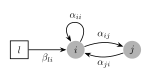
\includegraphics[width=0.8\textwidth]{modelli/modello influenza.pdf}
	\end{minipage}
	\begin{minipage}{0.5\textwidth}
		\begin{align*}
			l \;\; &\rightarrow \;\; \text{causa indipendente che influenza } i \\
			i,j  \;\; &\rightarrow \;\; \text{oggetti influenzati o influenzanti} \\
			\alpha, \beta\;\; &\rightarrow \;\; \text{parametri di influenza} \in \mathbb{R} 
		\end{align*}
	\end{minipage}
	\begin{align*}
		x_i(t/k) &\rightarrow \;\; \text{opinione del primo oggetto/persona, variabile di stato} \\
		x_j(t/k) &\rightarrow \;\; \text{opinione del secondo oggetto/persona, variabile di stato} \\
		\alpha_{ij} x_i(t/k) &\rightarrow \;\; \text{influenza di } i \text{ sull'oggetto } j \\
		\alpha_{ji} x_j(t/k) &\rightarrow \;\; \text{influenza di } j \text{ sull'oggetto } i \\
		\alpha_{ii} x_i(t/k) &\rightarrow \;\; \text{mantenimento della propria opinione} \\
		\beta_{li} u_l(t/k) &\rightarrow \;\; \text{influenza dall'ingresso indipendente } il \\
	\end{align*}
\end{center}

\subsubsection*{Rappresentazione in funzioni matematiche}
Per il tempo discreto si ottiene:
\[x_i(k+1) = \sum_{j=1}^{n} \alpha_{ji} x_j(k) + \sum_{l=1}^{p} \beta_{li} u_l(k) \qquad x(k+1) = Ax(k) + Bu(k) \quad a_{ij} = \alpha_{ji}\]
Per il tempo continuo si ottiene:
\[\dot{x}_i(t) = \sum_{j=1}^{n} \alpha_{ji} x_j(t) + \sum_{l=1}^{p} \beta_{li} u_l(t) \qquad \dot{x}(t) = Ax(t) + Bu(t) \quad a_{ij} = \alpha_{ji}\]
Esistono due modelli di influenza delle opinioni, per sistemi isolati, che hanno la particolarità di prevedere o meno l'influenza
dalle condizioni iniziali:
\begin{itemize}
	\item \textbf{modello di DeGroot}: lo stato non è influenzato dalla condizione iniziale e all'equilibrio tutti gli oggetti
	avranno la stessa opinione \[x(k+1) = \lambda A x(k) + (1-\lambda) \; x(0) \quad \lambda = 1 \quad \rightarrow \quad x(k+1) = A x(k)\]
	\item \textbf{modello di Friedkin e Johnsen}: lo stato è sempre influenzato dalla condizione iniziale e all'equilibrio le
	opinioni non convergono ad un consenso comune \[x(k+1) = \lambda A x(k) + (1-\lambda) \; x(0) \quad 0 \leq \lambda \leq 1\]
\end{itemize}

\newpage

\subsubsection*{Analisi qualitativa del diagramma delle fasi o spazio di stato}
Per risolvere i problemi di influenza si ricorre allo studio del diagramma delle fasi detto anche spazio di stato, ovvero del
grafico in cui, negli assi cartesiani sono presenti le variabili di stato e si è indipendenti dal tempo. Per semplicità si
scelgono solo modelli con due oggetti/persone e con ingressi costanti:
\begin{align*}
	&0 = \dot{x}_1(t) = \alpha_{11} x_1(t) + \alpha_{21} x_2(t) + \beta_{11} \bar{u}_1 + \beta_{21} \bar{u}_2 \\
	&0 = \dot{x}_2(t) = \alpha_{12} x_1(t) + \alpha_{22} x_2(t) + \beta_{12} \bar{u}_1 + \beta_{22} \bar{u}_2
\end{align*}
\begin{itemize}
	\item si analizzano le funzioni matematiche che descrivono il sistema all'equilibrio in maniera indipendente in modo da trovare
	delle equazioni che descrivono delle rette \(x_1 = m_1 x_2 + q_1\) e \(x_2 = m_2 x_1 + q_2\)
	\[x_1 = -\frac{\alpha_{21}}{\alpha_{11}} x_2 - \frac{\beta_{11} \bar{u}_1 + \beta_{21} \bar{u}_2}{\alpha_{11}} \qquad\qquad x_2 = -\frac{\alpha_{12}}{\alpha_{22}} x_1 - \frac{\beta_{12} \bar{u}_1 + \beta_{22} \bar{u}_2}{\alpha_{22}}\]
	\item si tracciano le rette nel diagramma delle fasi e si analizza il grafico ottenuto, se esiste il punto di equilibrio, allora
	è l'intersezione delle due rette
\end{itemize}

\subsubsection*{Esempi visti a lezione}
\begin{itemize}
	\item relazione amorosa tra Romeo e Giulietta
	\item corsa agli armamenti
	\item dinamica dei prezzi
\end{itemize}

\subsubsection*{Corsa agli armamenti a tempo continuo}
Sono presenti due nazioni che si influenzano a vicenda e due cause (aggressività delle nazioni) che influenzano rispettivamente
la prima e la seconda nazione.
\[\dot{x}_1(t) = -\alpha_{11} x_1(t) + \alpha_{21} x_2(t) + \bar{u}_1 \qquad x_1 = \frac{\alpha_{21}}{\alpha_{11}} x_2 + \frac{\bar{u}_1}{\alpha_{11}}\]
\[\dot{x}_2(t) = \alpha_{12} x_1(t) - \alpha_{22} x_2(t) + \bar{u}_2 \qquad x_2 = \frac{\alpha_{12}}{\alpha_{22}} x_1 + \frac{\bar{u}_2}{\alpha_{22}}\]

Per la corsa agli armamenti si era osservato che potevano verificarsi due casi, in base ai valori \(\alpha\):
\begin{itemize}
	\item[1.] le rette si incontrano nel punto di equilibrio e si divide il piano in 4 quadranti, analizzando i casi in cui \(\dot{x}_1(t) > 0\) e \(\dot{x}_2(t) > 0\)
	si osservava cosa avviene in ciascuno dei 4 quadranti: si tende all'equilibrio
	\item[2.] le rette non si incontrano e dividono il piano in 3 sezioni, analizzando cosa avveniva nelle tre sezioni si osserva che
	tra le due rette, il sistema diverge a \(+\infty\), altrimenti converge sulle due rette
\end{itemize}

\subsubsection*{Dinamica dei prezzi a tempo discreto}
Si definiscono i consumatori e i produttori con le loro sensibilità:
\[\begin{array}{l} q = b p + Q \\ q = -a p + D \end{array} \quad \begin{array}{l} p = \text{prezzo} \\ q = \text{quantità}\end{array} \quad \begin{array}{l} a = \text{sensib. consumatori} \\ b = \text{sensib. produttori}\end{array} \qquad \begin{array}{l} q(k) = -ap(k) + D \; \text{istantanea}\\ q(k\!+\!1) = bp(k) + Q \; \text{non istant.}\end{array}\]
Si analizza il grafico ottenuto dalle due rette in funzione dei parametri \(a, b\) e delle variabili di stato \(p, q\) e si
osserva che le rette sono sempre incidenti nel punto di equilibrio, ma si distinguono tre casi:
\begin{itemize}
	\item \(a > b\): scelto un punto sulle rette, si tende a convergere nell'intersezione attraverso moti oscillanti \say{rettangolari}
	esponenzialmente smorzati
	\item \(a = b\): scelto un punto sulle due rette, si ottiene un moto oscillante \say{rettangolare} costante, per cui non si
	raggiungerà mai l'equilibrio, a meno che non si parta proprio da esso
	\item \(a < b\): scelto un punto sulle due rette, si ottiene un moto oscillante \say{rettangolare} divergente, per cui non si
	raggiungerà mai l'equilibrio, a meno che non si parta proprio da esso
\end{itemize}
Tale analisi si ottiene analizzando il prezzo di equilibrio \(p_{eq} = -^1\!/\!_{(a+b)} \, (D-Q)\) e analizzando la deviazione del prezzo
rispetto all'equilibrio \(\tilde{p}(k+1) = -^b\!/\!_a \, \tilde{p(k)}\) con \(\tilde{p}(k) = p(k) - p_{eq}\).

\newpage


\subsection{Modelli fisici}
\subsubsection*{Circuiti elettrici}
Per modellare un circuito elettrico si utilizza un sistema matematico con i seguenti elementi:
\begin{itemize}
	\item \textbf{variabili di stato}: le tensioni dei condensatori e le correnti negli induttori
	\item \textbf{ingressi}: i vari generatori e disturbi
	\item \textbf{equazioni}: equazioni costitutive dei componenti e le leggi di Kirchhoff per il circuito
\end{itemize}

\subsubsection*{Sistemi meccanici traslazionali}
Per modellare i sistemi meccanici traslazionali (carrellino, molla, smorzatore) si definiscono:
\begin{itemize}
	\item \textbf{variabili di stato}: le posizioni e relative derivate dei carrellini/oggetti in movimento
	\item \textbf{ingressi}: le forze esterne agenti sul sistema
	\item \textbf{equazioni}: equazioni costitutive delle varie parti (molla, smorzatore), il primo principio della dinamica
	(inerzia) e il secondo principio (legge di Newton)
\end{itemize}

\subsubsection*{Sistemi meccanici rotativi}
Per modellare i sistemi meccanici rotativi (massa rotante, molla torsionale, smorzatore rotante) si definiscono:
\begin{itemize}
	\item \textbf{variabili di stato}: posizione angolare e relative derivate delle masse rotanti
	\item \textbf{ingressi}: momenti esterni agenti sul sistema
	\item \textbf{equazioni}: equazioni costitutive delle varie parti (molla torsionale e smorzatore torsionale), il primo
	principio della dinamica (inerzia) e il secondo principio (legge di Newton per rotazioni)
\end{itemize}

\subsection{Sistemi dinamici non lineari}
I sistemi fisici non lineari sono particolarmente ostici da analizzare dal punto vista matematico. Per cui, per studiarli, verranno
linearizzati attorno ai punti di equilibrio e ne verrà studiato il comportamento per brevi scostamenti dall'equilibrio.

\subsubsection*{Rappresentazione matematica di un sistema non lineare}
Il sistema non lineare non si può esprimere come combinazione lineare degli stati e degli ingressi/uscite, ma si utilizzano generiche
funzioni dipendenti dagli stati e dagli ingressi/uscite.
\begin{align*}
	&\text{tempo continuo} \quad \begin{cases} \dot{x}_1(t) = f_1 (x_1(t), \dots, x_n(t), u_1(t), \dots, u_m(t)) \\ \;\;\, \dots \; = \; \dots \\ \dot{x}_n(t) = f_n (x_1(t), \dots, x_n(t), u_1(t), \dots, u_m(t)) \end{cases} &\leftrightarrow \quad &\dot{x}(t) = f(x(t),u(t)) \\
	&\text{tempo discreto} \quad \begin{cases} x_1(k+1) = f_1 (x_1(k), \dots, x_n(k), u_1(k), \dots, u_m(k)) \\ \qquad\;\,\, \dots \; = \; \dots \\ x_n(k+1) = f_n (x_1(k), \dots, x_n(k), u_1(k), \dots, u_m(k)) \end{cases} &\leftrightarrow \quad &x(k+1) = f(x(k),u(k))
\end{align*}

\subsubsection*{Studio dell'equilibrio}
Si studiano le equazioni in modo da ottenere gli stati stazionari (tempo continuo) o i punti fissi (tempo discreto) tali per cui
si ha stabilità.
\begin{align*}
	&\text{tempo continuo} \quad \begin{cases} 0 = \dot{\bar{x}}_1(t) = f_1 (\bar{x}_1(t), \dots, \bar{x}_n(t), \bar{u}_1(t), \dots, \bar{u}_m(t)) \\ \qquad \dots \;\;\; = \;\;\; \dots \end{cases} \\
	&\text{tempo discreto} \quad \begin{cases} \bar{x}_1(k) = f_1 (\bar{x}_1(k), \dots, \bar{x}_n(k), \bar{u}_1(k), \dots, \bar{u}_m(k)) \\ \;\;\:\, \dots \; = \; \dots  \end{cases}
\end{align*}

\subsubsection*{Linearizzazione all'equilibrio}
Attraverso l'espansione di Taylor si linearizzano le funzioni intorno ai punti di equilibrio con:
\begin{itemize}
	\item \((\bar{x}_{eq},\bar{u}_{eq}) = (\bar{x}_1, \dots \bar{x}_n, \bar{u}_1, \dots, \bar{u}_m)\)
	\item \((\tilde{x},\tilde{u}) = (x,u)-(x_{eq},u_{eq}) \;\; \rightarrow \;\; (\tilde{x}_{eq},\tilde{u}_{eq}) = (\vec{0},\vec{0})\)
\end{itemize}

\vspace{10pt}
\noindent
Di seguito la linearizzazione di \(f_1\) in tempo continuo con Taylor, si osserva che si ottiene una combinazione lineare delle
variabili di stato e degli ingressi in cui i coefficienti sono ottenuti dalle derivate parziali.
\begin{align*}
	\dot{x}_1(t) &= f_1(x_1(t), \dots x_n(t), u_1(t), \dots, u_m(t)) = \\
	\dot{x}_1(t) &\approx \underbrace{f_1(\bar{x}_1, \dots \bar{x}_n, \bar{u}_1, \dots, \bar{u}_m)}_{=0} + \underbrace{ \left. \frac{\partial f_1}{\partial x_1} \right|_{\bar{x}, \bar{u}} }_{{a_{11}}} \underbrace{ \left( x_1(t) - \bar{x}_1 \right) }_{\tilde{x}_1} + \cdots + \underbrace{ \left. \frac{\partial f_1}{\partial x_n} \right|_{\bar{x}, \bar{u}} }_{a_{1n}} \underbrace{ \left( x_n(t) - \bar{x}_n \right) }_{\tilde{x}_n} + \\
	&\qquad\qquad\qquad\qquad\qquad\qquad + \underbrace{ \left. \frac{\partial f_1}{\partial u_1} \right|_{\bar{x}, \bar{u}} }_{{b_{11}}} \underbrace{ \left( u_1(t) - \bar{u}_1 \right) }_{\tilde{u}_1} + \cdots + \underbrace{ \left. \frac{\partial f_1}{\partial u_m} \right|_{\bar{x}, \bar{u}} }_{b_{1m}} \underbrace{ \left( u_m(t) - \bar{u}_m \right) }_{\tilde{u}_m} \\
	\dot{x}_1(t) &\approx a_{11} \tilde{x}_1 + \dots + a_{1n} \tilde{x}_n + b_{11} \tilde{u}_1 + \dots + b_{1m} \tilde{u}_m
\end{align*}

\[\text{In generale} \qquad \dot{\tilde{x}}(t) \approx A \tilde{x}(t) + B \tilde{u}(t) \qquad\qquad A = (a_{ij}) \quad a_{ij} = \left. \frac{\partial f_i}{\partial x_j} \right|_{\bar{x}, \bar{u}} \qquad B = (b_{ij}) \quad b_{ij} = \left. \frac{\partial f_i}{\partial u_j} \right|_{\bar{x}, \bar{u}}\]

\vspace{10pt}
\noindent
Di seguito la linearizzazione di \(f_1\) in tempo discreto con Taylor, si osserva che si ottiene una combinazione lineare delle
variabili di stato e degli ingressi in cui i coefficienti sono ottenuti dalle derivate parziali.
\begin{align*}
	x_1(k+1) &= f_1(x_1(k), \dots x_n(k), u_1(k), \dots, u_m(k)) = \\
	x_1(k+1) &\approx \underbrace{f_1(\bar{x}_1, \dots \bar{x}_n, \bar{u}_1, \dots, \bar{u}_m)}_{=0} + \underbrace{ \left. \frac{\partial f_1}{\partial x_1} \right|_{\bar{x}, \bar{u}} }_{{a_{11}}} \underbrace{ \left( x_1(k) - \bar{x}_1 \right) }_{\tilde{x}_1} + \cdots + \underbrace{ \left. \frac{\partial f_1}{\partial x_n} \right|_{\bar{x}, \bar{u}} }_{a_{1n}} \underbrace{ \left( x_n(k) - \bar{x}_n \right) }_{\tilde{x}_n} + \\
	&\qquad\qquad\qquad\qquad\qquad\qquad + \underbrace{ \left. \frac{\partial f_1}{\partial u_1} \right|_{\bar{x}, \bar{u}} }_{{b_{11}}} \underbrace{ \left( u_1(k) - \bar{u}_1 \right) }_{\tilde{u}_1} + \cdots + \underbrace{ \left. \frac{\partial f_1}{\partial u_m} \right|_{\bar{x}, \bar{u}} }_{b_{1m}} \underbrace{ \left( u_m(k) - \bar{u}_m \right) }_{\tilde{u}_m} \\
	x_1(k+1) &\approx a_{11} \tilde{x}_1 + \dots + a_{1n} \tilde{x}_n + b_{11} \tilde{u}_1 + \dots + b_{1m} \tilde{u}_m
\end{align*}

\[\text{In generale} \qquad \tilde{x}(k+1) \approx A \tilde{x}(k) + B \tilde{u}(k) \qquad\quad A = (a_{ij}) \quad a_{ij} = \left. \frac{\partial f_i}{\partial x_j} \right|_{\bar{x}, \bar{u}} \qquad B = (b_{ij}) \quad b_{ij} = \left. \frac{\partial f_i}{\partial u_j} \right|_{\bar{x}, \bar{u}}\]
